%!TEX root = ../thesis.tex

\section{セグメンテーションによる処理速度の問題}
第3章で述べた提案手法は，リアルタイム性を向上するゼロショットセグメンテーションを実現する一方で，処理速度（FPS）が十分に得られないという課題がある．特に，SAM2は大規模なモデルであり，毎フレーム実行すると処理速度が低下し，リアルタイム性が損なわれる可能性がある．この問題を解決するために，本章では提案手法の改良について検討する．

\vspace{1cm}

\begin{figure}[H]
\centering
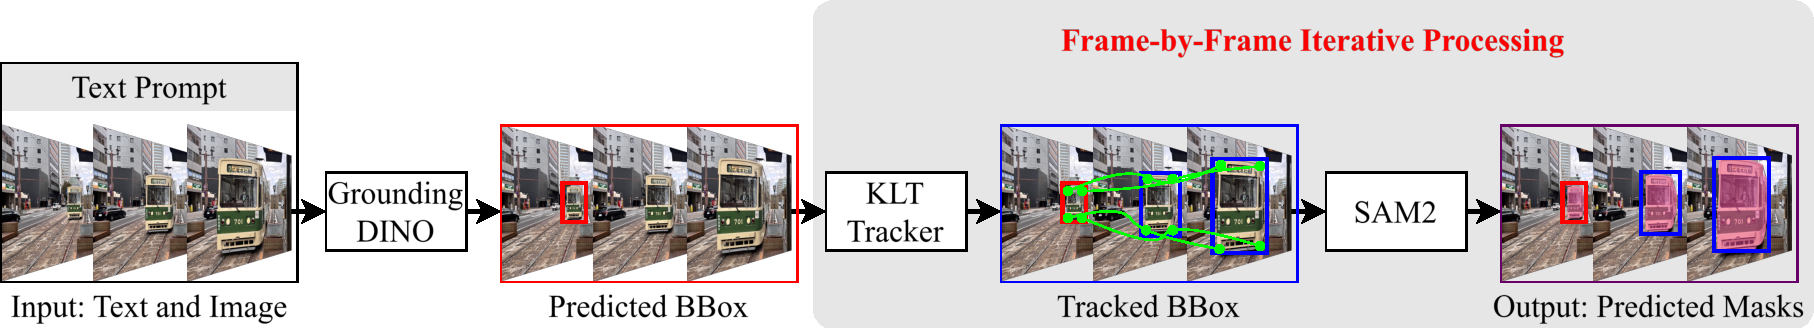
\includegraphics[width=1.0\linewidth]{images/pdf/system_problem.pdf}
\caption{Problem of processing speed due to segmentation.}
\label{fig:system_problem}
\end{figure}

\newpage

\section{さらなる高速化に向けた提案手法の処理}
さらなる高速化に向けた提案手法の処理について述べる．\Fig{fig:system_ver2}に示すように，さらなる高速化に向けた提案手法の処理は，(1) 物体検出およびセグメンテーション(2) 物体追跡，の 2 つの処理で構成される．以下にそれぞれの処理に関して述べる．

\begin{figure}[H]
\centering
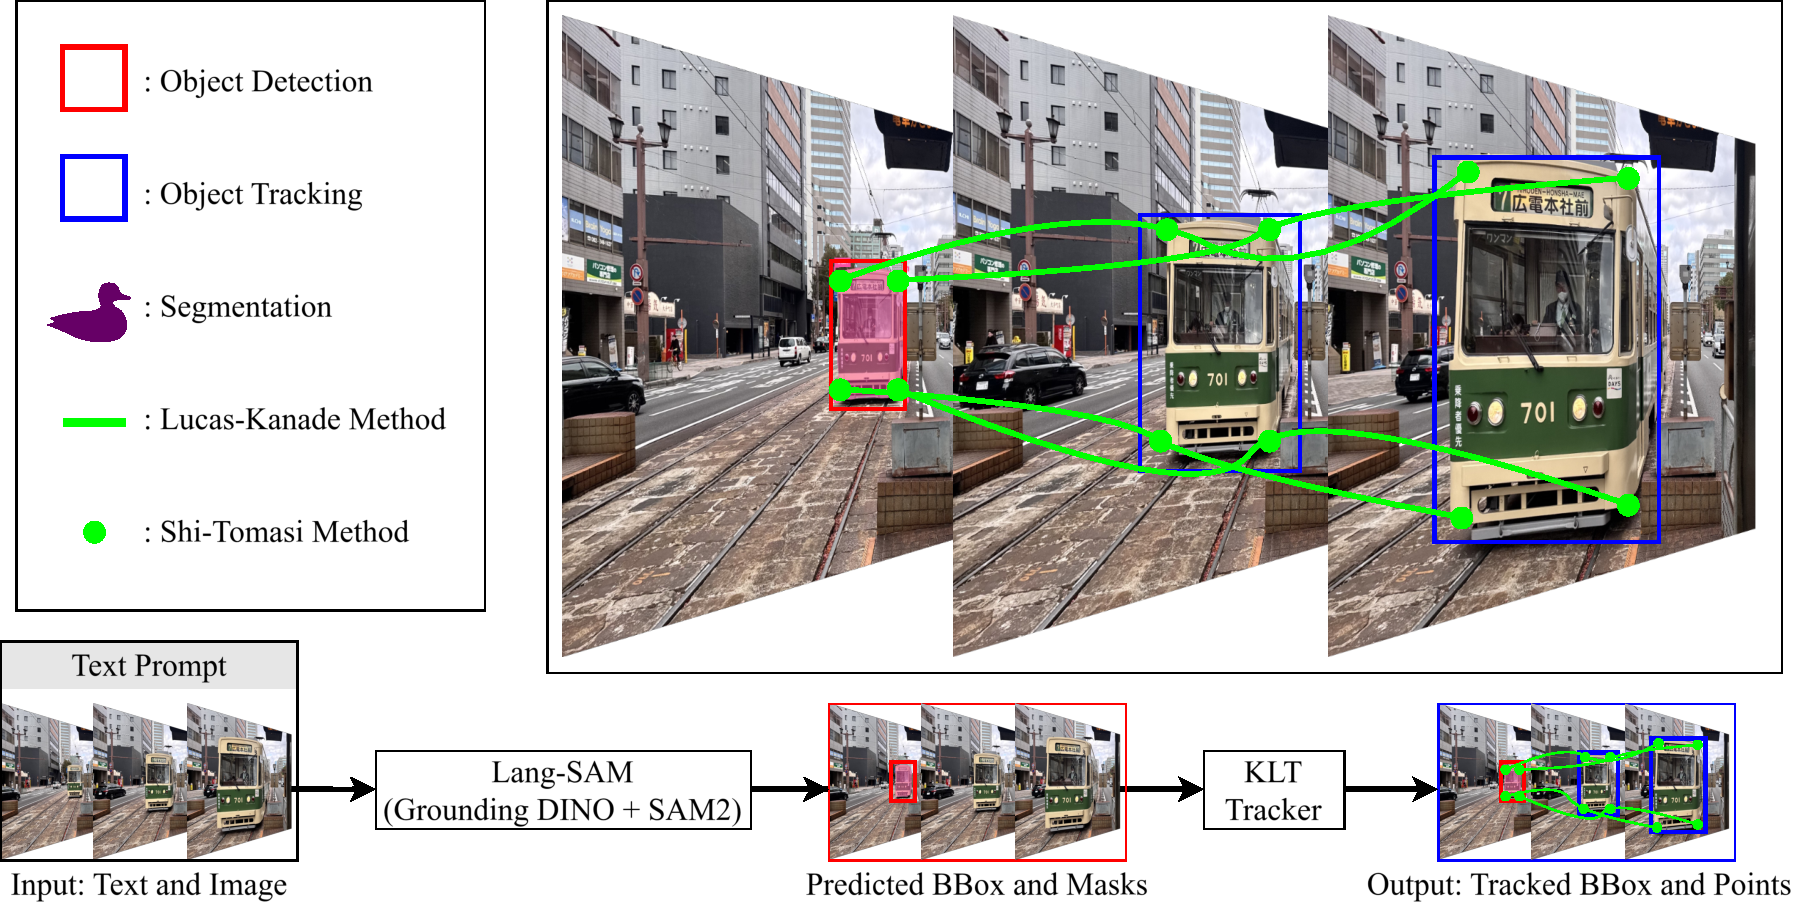
\includegraphics[width=1.0\linewidth]{images/pdf/system_ver2.pdf}
\caption{Overview of the improved system.}
\label{fig:system_ver2}
\end{figure}

\subsection{物体検出およびセグメンテーション}
テキストプロンプトに基づき，Grounding DINOを用いて物体検出を行う．これによって，テキストに対応するバウンディングボックス（BBox）が生成される．さらに，検出されたBBoxに対し，SAM2を用いてセグメンテーションマスクを生成する．この処理は，毎フレームではなく一定間隔で実行し，計算負荷が過大とならないようにする．

\newpage

\subsection{物体追跡}
後続のフレームでは，毎フレームGrounding DINOやSAM2を実行する代わりに，物体追跡でBBoxとPointsを更新する．まず，前フレームのセグメンテーション内でShi-Tomasi法 に基づき画像特徴点を抽出する．次に，抽出した特徴点群をLucas-Kanade法 に基づくピラミッドオプティカルフローで追跡し，その移動ベクトルの中央値を算出する．このベクトルを用いてBBoxの位置と大きさを更新する．以上の一連の処理を繰り返し実行する．これらの手法は，標準的かつ計算効率に優れていることから，特徴点追跡に採用した．これにより，検出とセグメンテーション，追跡までの一連の処理を行う．また，追跡した特徴点群を膨張または複製することで，セグメンテーションマスクのように扱うことが可能である．

\subsection{変更点のまとめ}
第3章で提案した手法と本章で提案した手法の比較を\Fig{fig:comparison}に示す．セグメンテーション処理を物体検出と同じタイミングで実行するように変更した．これにより，セグメンテーション処理の頻度が低減され，システム全体の処理速度が向上することが期待される．

\begin{figure}[H]
\centering
\begin{minipage}{1.0\linewidth}
\centering
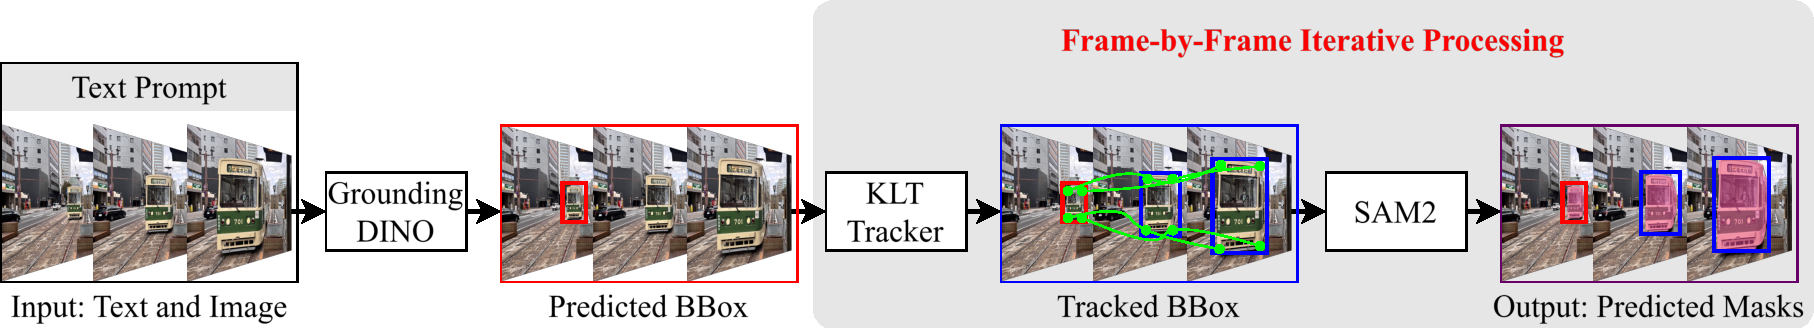
\includegraphics[width=1.0\linewidth]{images/pdf/system_problem.pdf}
\subcaption{Chapter 3 proposed method}
\label{fig:comparison_ch3}
\end{minipage}
\begin{minipage}{1.0\linewidth}
\centering
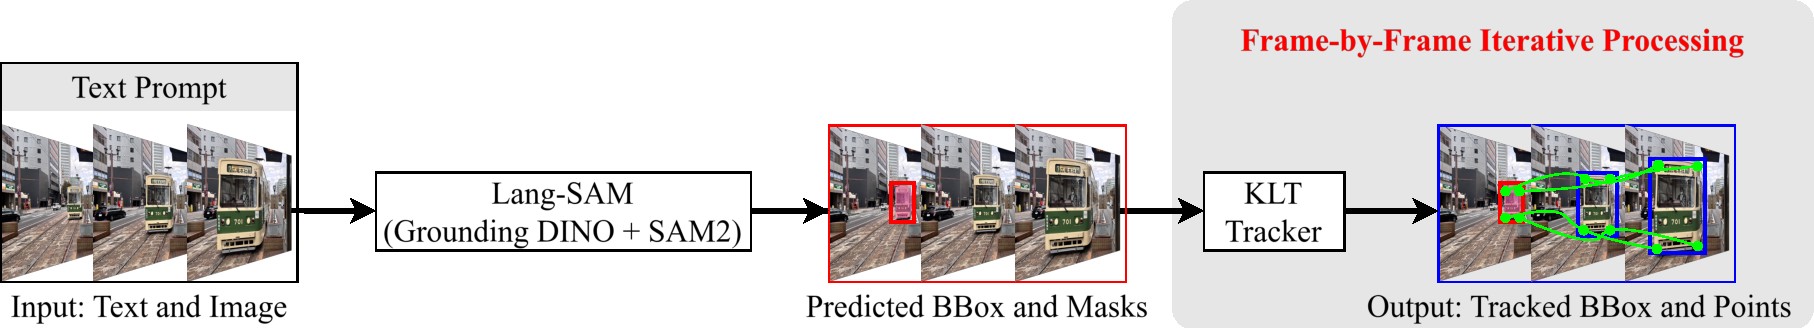
\includegraphics[width=1.0\linewidth]{images/pdf/system_process.pdf}
\subcaption{Improved method in this chapter}
\label{fig:comparison_improved}
\end{minipage}
\caption{Comparison between the proposed method in Chapter 3 and the improved method in this chapter.}
\label{fig:comparison}
\end{figure}

